\chapter{Basic concepts}
Spot essentially manipulates $\omega$-automata which is a variation of finite-state automata (FSA) that runs
on infinite, rather than finite. It is important to have a good understanding of automata theory,
not only to understand this report but because automata crop up preety much everywhere in computer
science. In logic design, natural language processing, system analysis, regular expressions, etc. The next
two sections introduce the basics of automata theory and some concepts used in Spot.

\section{Automata theory}
\textit{Automata theory} \cite{9} is the study of abstract machines and automata, as well as the
computational problems that can be solved using them.

\begin{figure}[H]
 \centering
 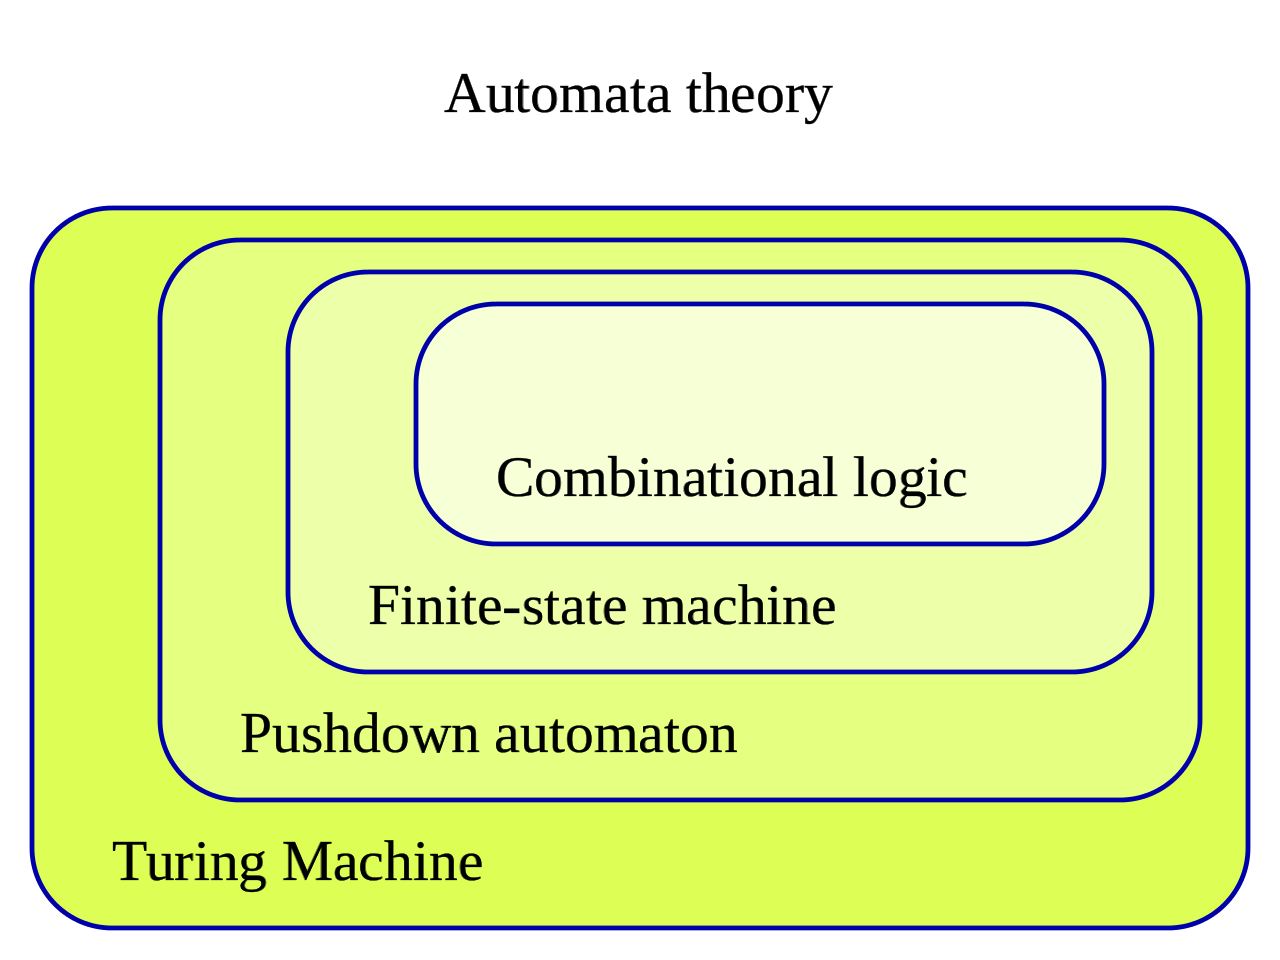
\includegraphics[scale=0.2]{img/automata_classes.png}
 \caption{Classes of automata \cite{9}}
 \label{fig:aut_classes}
\end{figure}
There are different classes of automata. The finite state machine has less computational power than
some other models of computation such as the Turing machine \cite{10}. The computational power distinction
means there are computational tasks that a Turing machine can do but a finite-state automaton (FSA) can
not.\\

\noindent From now on, the acronym FSA will be used instead of final-state automat\{a, on\}.\\

Only FSA will be concisely described in this section as (again) $\omega$-automata used in Spot are a
variation of FSA.

\subsection{Automata}
\begin{figure}[h]
  \centering
  \begin{tikzpicture}[shorten >=1pt,node distance=4cm,on grid,auto] 
    \node[state,initial] (q_0)   {$q_0$};
    \node[state, accepting] (q_1) [right=of q_0] {$q_1$};
    \path[->] 
    (q_0) edge[bend right=-30] node {$b$} (q_1)
          edge[loop above]     node {$a$} ()
    (q_1) edge[bend left=30]   node {$a$} (q_0)
          edge[loop above]     node {$b$} ();
  \end{tikzpicture}
  \caption{A finite-state automaton represented using a graph}
   \label{aut:pres}
\end{figure}

The figure (\ref{aut:pres}) shows how an automaton looks like. It consists of:
\begin{itemize}
 \item a set of states (represented in the figure by circles). Among them we can distinguish the 
       \textit{initial state} \textbf{q0} (the one pointed by \textbf{start}) and an
       \textit{accepting state} \textbf{q1} (the one doubly encircled).
 \item a transition relation (represented in the figure by arrows). This relation indicates for each
       state which state could be next according to the next symbol to read.
\end{itemize}

Before giving a regular definition, some points need clarification.

\subsection{Alphabet, word, language}
An alphabet is a finite set of symbols. It is commonly denoted by $\Sigma$. Edges of automata are labeled
by those symbols. The alphabet used by the automaton of figure \ref{aut:pres} is $\{a, b\}$. \\

\noindent A word is a finite sequence of symbols. $a$, $b$, $ab$, $aaaa$, $abbba$, $ababababbbaaabbaba$ are
some words defined on the alphabet $\{a, b\}$. Automata recognizes words. In Spot, $\omega$-automata
recognizes \textit{$\omega$-words}, which are infinite rather than finite.\\

\noindent A language is a set of words defined on the same alphabet. The automata of figure \ref{aut:pres}
accepts or recognizes the set of words ending with $b$. \textbf{q1} is the only one accepting state and
the only way to come in \textbf{q1} is to read b.

\subsection{Automaton run}
Well, an automaton run can be described as follows:
\begin{itemize}
 \item it starts in the initial state and waits for the first character (of the word) to read.
 \item At each step, it reads the next symbol (character) and determine the next state using the
       transition relation.
 \item It stops when all the character chain has been read. The word is accepted if the automaton is
       in one of the accepting states.
\end{itemize}

\subsection{Determinism (DFA, NFA)}
A \textit{deterministic} FSA is a final state machine where for each pair of state and input (symbols)
there is one and only one transition to a next state. The figure \ref{aut:pres} introduced before is
actually a \textit{deterministic} FSA or \textit{deterministic} finite-state automaton (DFA).\\

\noindent A \textit{non deterministic} FSA or \textit{Nondeterministic} finite-state automaton (NFA) allows:
\begin{itemize}
 \item many transitions labeled by the same symbol and outgoing from the same state,
 \item transitions labeled by the \textit{empty word} $\varepsilon$,
 \item transitions labeled by more than one symbol.
\end{itemize}

\subsection{Finite-state automata (FSA) Definition}
More formally, a finite-state automaton is defined by a quintuplet $M=(Q, \Sigma, X, s, F)$ where:
\begin{itemize}
 \item $Q$ is a set of states,
 \item $\Sigma$ is an alphabet,
 \item $X$ can be either a transition function $\delta : Q \times \Sigma \rightarrow Q$ (if the automaton is
       deterministic) or a transition relation $\Delta \subset (Q \times \Sigma^* \times Q)$ (if it is not
       deterministic),
 \item $s \in Q$ is the initial state,
 \item $F \subseteq Q$ is a set of accepting states.
\end{itemize}

\section{About Spot}
This section consists essentially of Spot's \textbf{concept} web page excerpts\cite{8}. Feel free to have a
look on that web page for further details.

\subsection{Atomic preposition}
An \textit{atomic proposition} is a named Boolean variable that represents a simple property that must be
true or false. It usually represents some property of a system. They are used to construct temporal logic
formulas\cite{13} to specify properties of the system.

\subsection{Boolean formula}
A Boolean formula is formed from \textit{atomic preposition}, the Boolean constants true and false, and
standard Boolean operators like and, or, implies, xor, etc.

\subsection{$\omega$-words}
An $\omega$-word as said before is a word of infinite length. In our context, each letter is used to
describe the state of a system at a given time, and the sequence of letters shows the evolution of the
system as the (discrete) time is incremented.\\

If the set \textbf{AP} of atomic propositions is fixed, an $\omega$-word over \textbf{AP} is an infinite
sequence of subsets of \textbf{AP}. In other words, there are 2$^{|\textbf{AP}|}$ possible letters to
choose from, and these letters denote the set of atomic propositions that are true at a given instant.\\

For instance if \textbf{AP}$=\{a,b,c\}$, the infinite sequence $\{a,b\}$;$\{a\}$;$\{a,b\}$;$\{a\}$;
$\{a,b\}$;$\{a\}$;… is an example of $\omega$-word over \textbf{AP}. This particular $\omega$-word can be
interpreted as the following scenario: atomic proposition $a$ is always true, $b$ is true at each other
instant, and $c$ is always false.

\subsection{$\omega$-automaton}
An $\omega$-automaton is used to represent sets of $\omega$-word.\\

Those look like the classical NFA in the sense that they also have states and transitions. However
$\omega$-automata recognize $\omega$-words instead of finite words. In this context, the notion of final
state makes no sense, and is replaced by the notion of acceptance condition: a run of the automaton
(i.e., an infinite sequence alternating states and edges in a way that is compatible with the structure of
the automaton) is accepting if it satisfies the constraint given by the acceptance condition.\\

In Spot, $\omega$-automata have their edges labeled by Boolean formulas. An $\omega$-word is accepted by an
$\omega$-automaton if there exists an accepting run whose labels (those Boolean formulas) are compatible
with the minterms \cite{11} used as letters in the word.\\

The language of an $\omega$-automaton is the set of $\omega$-words it accepts.\\

There are many kinds of $\omega$-automata and they mostly differ by their acceptance condition. The
different types of acceptance condition, and whether the automata are deterministic or not can affect their
expressive power.

\begin{figure}[H]
 \centering
 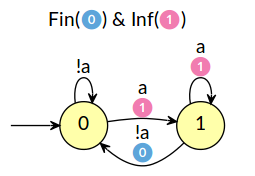
\includegraphics[scale=0.8]{img/omega_aut.png}
 \caption{$\omega$-automaton representing formula \textbf{FGa}}
 \label{fig:omega_aut}
\end{figure}

\subsection{Acceptance condition}
An acceptance condition actually consists of two pieces: some acceptance sets, and a formula that tells
how to use these acceptance sets.\\

Acceptance formulas are positive Boolean formula over atoms of the form $t$, $f$, $Inf(n)$, or $Fin(n)$,
where $n$ is a non-negative integer denoting an acceptance set.
\begin{itemize}
 \item $\textbf{t}$ denotes the true acceptance condition: any run is accepting
 \item $\textbf{f}$ denotes the false acceptance condition: no run is accepting
 \item $\textbf{Inf(n)}$ means that a run is accepting if it visits infinitely often the acceptance set n
 \item $\textbf{Fin(n)}$ means that a run is accepting if it visits finitely often the acceptance set n
\end{itemize}

The above atoms can be combined using only the operator $\&$ and $|$ (also known as $\land$ and $\lor$), and
parentheses for grouping. Note that there is no negation, but an acceptance condition can be negated
swapping $t$ and $f$, $\land$ and $\lor$, and $Fin(n)$ and $Inf(n)$.\\

The following table gives an overview of how some classical acceptance condition are encoded. The first
column gives a name that is more human readable (those names are defined in the HOA \cite{3} format and
are also recognized by Spot). The second column give the encoding as a formula. Everything here is
case-sensitive.

\begin{figure}[H]
 \centering
 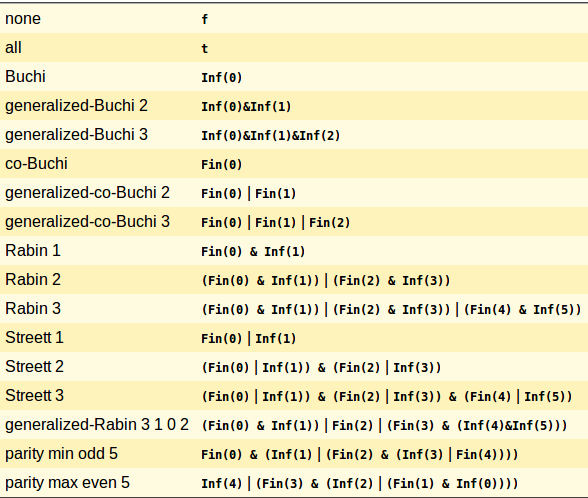
\includegraphics[scale=0.6]{img/acc_conds.png}
 \caption{$\omega$-automata acceptance conditions \cite{8}}
 \label{fig:acc_conds}
\end{figure}

\section{SAT solver}
Satisfiability problem is a classic of computer science.\\

The purpose of SAT solving is to assign each variables of a propositional formula in such a way that the
formula evaluates to true. It is the canonical NP-complete problem. SAT solvers are used to solve many
practical problems and this is also the case in Spot, they are used to minimize $\omega$-automata.\\

For more details, \textbf{SAT-solving in practice} \cite{16} is a good introduction to SAT solvers.